
\documentclass[a4paper,UKenglish,cleveref, autoref, thm-restate]{lipics-v2021}
%This is a template for producing LIPIcs articles. 
%See lipics-v2021-authors-guidelines.pdf for further information.
%for A4 paper format use option "a4paper", for US-letter use option "letterpaper"
%for british hyphenation rules use option "UKenglish", for american hyphenation rules use option "USenglish"
%for section-numbered lemmas etc., use "numberwithinsect"
%for enabling cleveref support, use "cleveref"
%for enabling autoref support, use "autoref"
%for anonymousing the authors (e.g. for double-blind review), add "anonymous"
%for enabling thm-restate support, use "thm-restate"
%for enabling a two-column layout for the author/affilation part (only applicable for > 6 authors), use "authorcolumns"
%for producing a PDF according the PDF/A standard, add "pdfa"

%\pdfoutput=1 %uncomment to ensure pdflatex processing (mandatatory e.g. to submit to arXiv)
\hideLIPIcs  %uncomment to remove references to LIPIcs series (logo, DOI, ...), e.g. when preparing a pre-final version to be uploaded to arXiv or another public repository

%\graphicspath{{./graphics/}}%helpful if your graphic files are in another directory

\bibliographystyle{plainurl}% the mandatory bibstyle

\title{PACE Solver Description: The SOAP1 Algorithm} %TODO Please add

\titlerunning{The SOAP1 Algorithm} %TODO optional, please use if title is longer than one line

%TODO mandatory, please use full name; only 1 author per \author macro; first two parameters are mandatory, other parameters can be empty. Please provide at least the name of the affiliation and the country. The full address is optional
\author{Christopher Weyand}{Karlsruhe Institute of Technology, Karlsruhe, Germany}{christopher.weyand@kit.edu}{https://orcid.org/0000-0003-0354-6650}{}
\author{Marcus Wilhelm}{Karlsruhe Institute of Technology, Karlsruhe, Germany}{marcus.wilhelm@kit.edu}{https://orcid.org/0000-0002-4507-0622}{}

\authorrunning{C. Weyand and M. Wilhelm} %TODO mandatory. First: Use abbreviated first/middle names. Second (only in severe cases): Use first author plus 'et al.'

\Copyright{Christopher Weyand and Marcus Wilhelm} %TODO mandatory, please use full first names. LIPIcs license is "CC-BY";  http://creativecommons.org/licenses/by/3.0/

\ccsdesc[100]{Mathematics of computing $\rightarrow$ Graph algorithms} %TODO mandatory: Please choose ACM 2012 classifications from https://dl.acm.org/ccs/ccs_flat.cfm 

\keywords{twinwidth} %TODO mandatory; please add comma-separated list of keywords

%\category{} %optional, e.g. invited paper

%\relatedversion{} %optional, e.g. full version hosted on arXiv, HAL, or other respository/website
%\relatedversiondetails[linktext={opt. text shown instead of the URL}, cite=DBLP:books/mk/GrayR93]{Classification (e.g. Full Version, Extended Version, Previous Version}{URL to related version} %linktext and cite are optional

\supplement{The source code is available on GitHub (\url{https://github.com/chistopher/twinwidth}) and Zenodo (\url{https://doi.org/10.5281/zenodo.7989779}).}%optional, e.g. related research data, source code, ... hosted on a repository like zenodo, figshare, GitHub, ...
%\supplementdetails[linktext={opt. text shown instead of the URL}, cite=DBLP:books/mk/GrayR93, subcategory={Description, Subcategory}, swhid={Software Heritage Identifier}]{General Classification (e.g. Software, Dataset, Model, ...)}{URL to related version} %linktext, cite, and subcategory are optional

%\funding{(Optional) general funding statement \dots}%optional, to capture a funding statement, which applies to all authors. Please enter author specific funding statements as fifth argument of the \author macro.

%\acknowledgements{I want to thank \dots}%optional

\nolinenumbers %uncomment to disable line numbering


%Editor-only macros:: begin (do not touch as author)%%%%%%%%%%%%%%%%%%%%%%%%%%%%%%%%%%
\EventEditors{John Q. Open and Joan R. Access}
\EventNoEds{2}
\EventLongTitle{42nd Conference on Very Important Topics (CVIT 2016)}
\EventShortTitle{CVIT 2016}
\EventAcronym{CVIT}
\EventYear{2016}
\EventDate{December 24--27, 2016}
\EventLocation{Little Whinging, United Kingdom}
\EventLogo{}
\SeriesVolume{42}
\ArticleNo{23}
%%%%%%%%%%%%%%%%%%%%%%%%%%%%%%%%%%%%%%%%%%%%%%%%%%%%%%

\begin{document}

\maketitle

%TODO mandatory: add short abstract of the document
\begin{abstract}
Twinwith is a recently introduced graph parameter that sparked a large body of algorithmic results as well as structural insights.
The parameter is bounded on important graph classes and enables FPT-algorithms for many hard problems.
Although computing the exact twinwidth of a graph is NP-hard, we present an algorithm that is able to compute the twinwith of small to medium sized graphs in practice.
In this write-up we outline the core techniques used in our exact twinwidth algorithm submitted to the exact track of the 2023 PACE challenge.
\end{abstract}

\section{Preliminaries}
The concept of twinwidth captures the distance of a graph to a co-graph~\cite{twin1}.
In this section we give a brief definition.

We define a \emph{contraction} (or \emph{merge}) of two vertices $u,v$ in a simple and undirected graph as follows.
The two vertices are deleted from the graph and replaced by a new vertex $w$.
For all other vertices $x$, $w$ has an edge to $x$ if both, $u$ and $v$ had an edge to $x$.
Similarly, $w$ has no edge to $x$ if both $u$ and $v$ had no edge to $x$.
In all other cases $w$ and $x$ are connected by a \emph{red edge}.
For the purpose of a contraction, red edges are considered as neither edges nor non-edges.
The \emph{red degree} of a vertex is the number of adjacent red edges.
The \emph{red degree} of a graph is the maximum red degree of its vertices.
The \emph{width} of a sequence of contractions is the maximum red degree of its intermediate graphs.
The \emph{twinwidth} of a graph is the minimum width over all contraction sequences that contract the graph into a single vertex.

\section{Solver Summary}
At its core, our solver is a branch-and-bound algorithm that finds an optimal contraction sequence.
It starts with an empty contraction sequence, applies reduction rules, and then branches on all possible merges.
After solving all branches recursively, the best one gives the result.
The algorithm maintains the best solution found so far as an upper bound for the input instance.
When a merge results in a width that is higher or equal to this upper bound then the current branch is pruned, since this branch cannot cannot contain a better solution.

The input instance is split into connected components which are solved separately.
This split is only done at the top-level call, because merges cannot separate components.


\subsection{Skip Seen Partitions}
In an intermediate graph after some contractions, each vertex represents a set of original vertices that were contracted to form this (super-)vertex.
Thus, the vertices of an intermediate graph imply a partitioning of the original vertices.
In fact, this partitioning uniquely defines the intermediate graph.
A crucial improvement of our algorithm is based on the observation that there are many partial contraction sequences that result in the same partitioning.
For example, doing the same contractions in a different order results in the same intermediate graph, however it might increase the width of the sequence.
The algorithm saves all partitions that are reached with a certain width.
If a partition is encountered that was previously reached with a lower or equal width, then the branch is pruned because any possible solution in this branch would also have been found the first time this partition was processed.
Since the twinwidth is less than $n$, the search-space of the algorithm is at most $n$ times the number of partitions of a set (also called the Bell number).


\subsection{Branching Strategy}
To find good upper bounds early, we process the branches in a certain order.
For each possible merge, we count the number of new red edges it creates.
Note that this number can be negative if two red edges fall together.
We process the branches that produce the least number of red edges first.


\subsection{Reduction Rules}
\begin{figure}
\centering
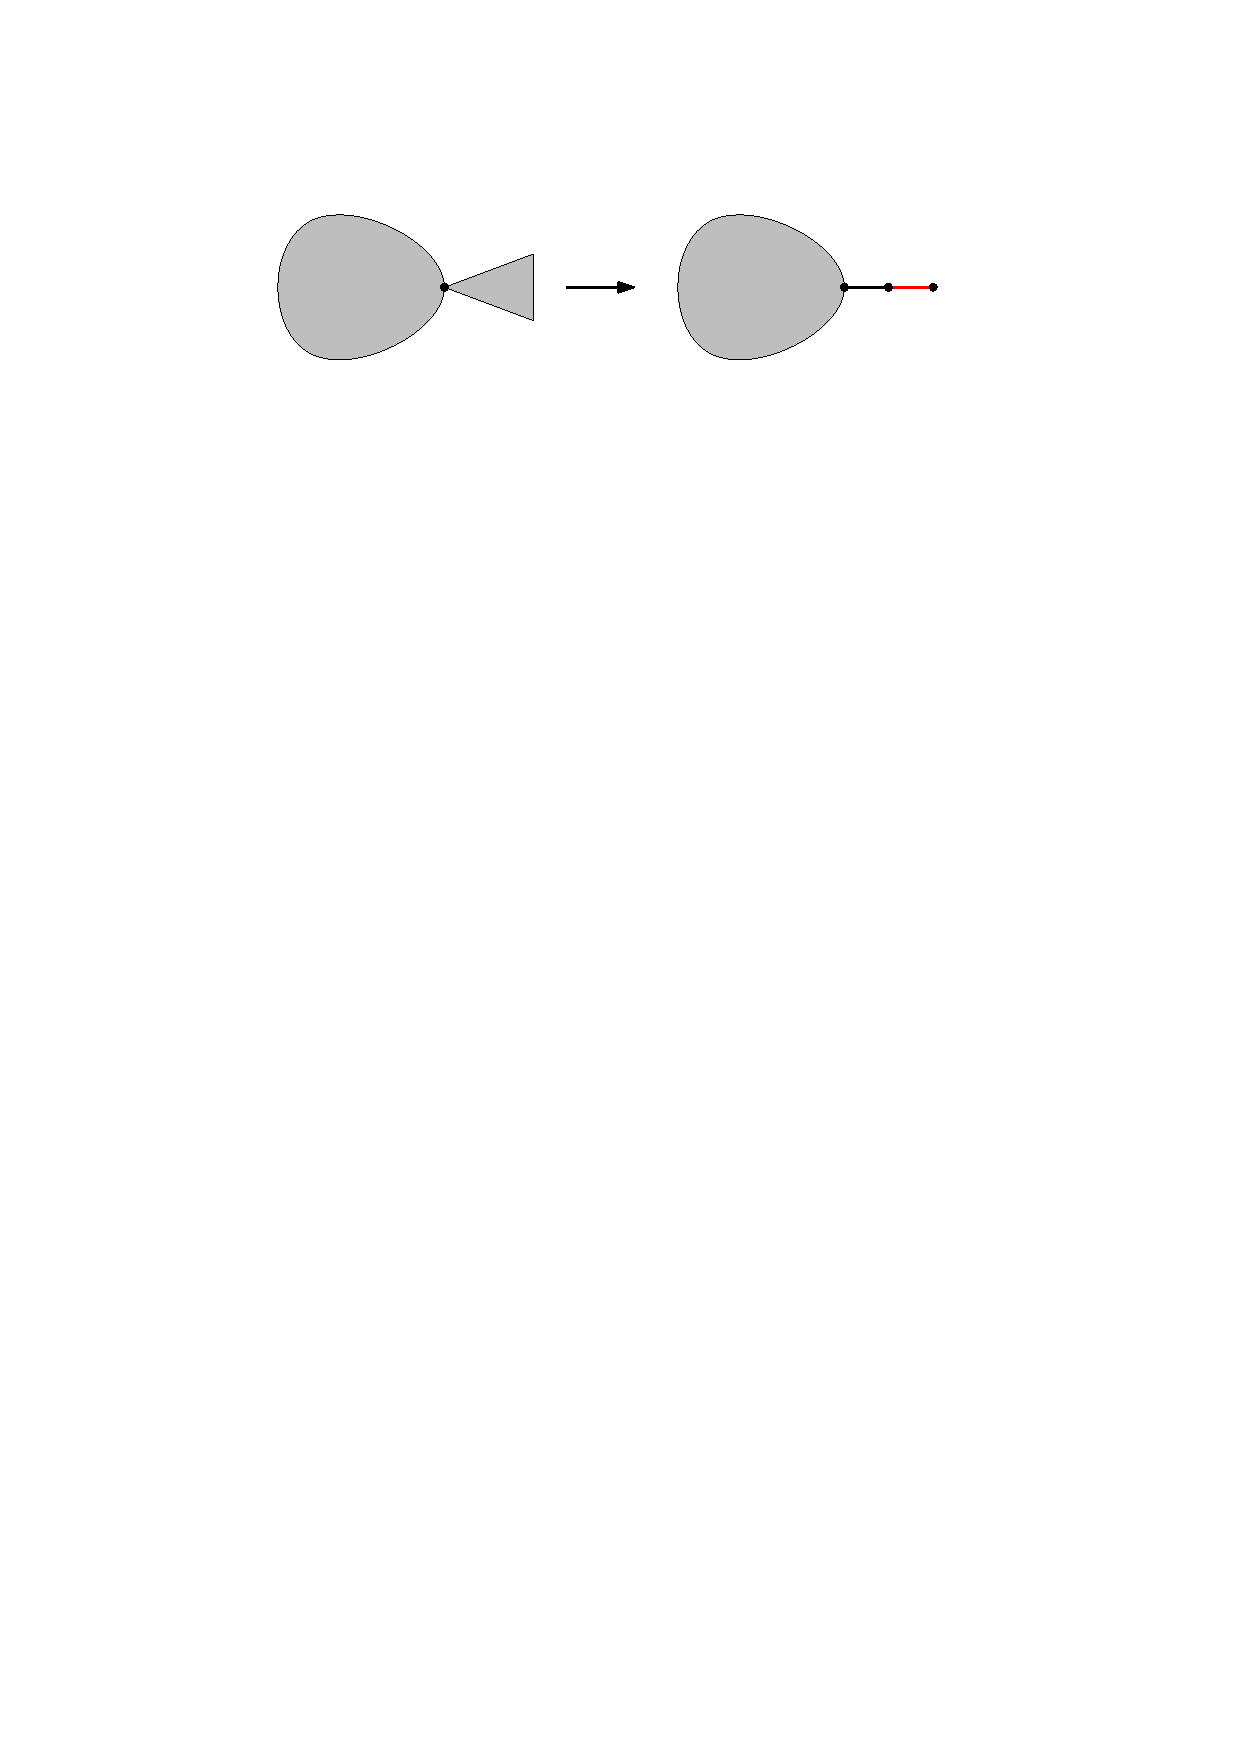
\includegraphics{cut}
\caption{The reduction rule to merge components behind a cut vertex. Proof: just trust me :)}
\label{fig:cut}
\end{figure}
We employ two reduction rules.
The first reduction rule is based on twins.
If the graph contains two distinct vertices with the same neighborhood, one of those vertices can be removed, because a merge of the two vertices has the same result as the removal of one of them and twinwidth is non-increasing for subgraphs.
To generalize this rule to red edges, we also consider two vertices twins, if the red edges of one vertex are a superset of the red edges of the other vertex and they agree on the neighbors for which neither has a red edge.
In this case, a merge would also be the same as the removal of the vertex with less red edges.

The second reduction rule aims to solve small biconnected components.
If a cut vertex separates a small component from the rest of the graph we try to heuristically merge the attached component into two vertices.
For this, we merge all direct neighbors of the cut vertex into one vertex and the rest of the component (if existing) into another vertex.
The result is shown in Figure~\ref{fig:cut}.
We can only apply the rule if the greedy merge does not increase the width.
That is, if the maximum red degree produced while merging the component is smaller or equal than a lower bound for the current instance.
The lower bound is obtained from the initial input instance or by the width of the partial contraction sequence so far.


\subsection{Lower Bounds}
Lower bounds are key to solving most instances.
If the lower bound matches the optimal solution, then the solver can stop as soon as such a solution is found.
If the lower bound is not tight, then the solver has to traverse the complete search space to prove optimality.
Most instances admit a huge number of optimal solutions and partial sequences that do not exceed the optimal width.
In general, it is way easier to find a good solution than to prove optimality.
Therefore, we made a great effort to find tight lower bounds.

The first type of bounds is based on the fact that the twinwidth is monotone w.r.t. taking subgraphs.
To obtain a lower bound for an instance, we find small subgraphs using various heuristics and solve them optimally using our solver.
We brute-force subgraphs of size 20-30 because they can be solved within few milliseconds.
Moreover, the public instances with a small twinwidth often have a small subgraph with the same width.
Unfortunately, we cannot obtain lower bounds that are higher than what is possible with 20-30 vertices.
E.g., random graphs have a twinwidth close to $n/2$~\cite{ahn2022twinwidth}.

The second type of lower bound is a look ahead.
Out of all possible merges, the one that results in the lowest width gives a lower bound.
This bound is zero if the graph has a twin but in turn can be quite high on random graphs (or after reductions).
We further combine this bound with the subgraph insight.
We iteratively delete a vertex that has a cheap merge while computing the look ahead bound after each step.
This results in a series of lower bounds for subgraphs, thus also lower bounds for the original instance.
The idea behind the bound is that the easy parts of the instance are deleted and we are left with a subgraph in which each merge results in high width.


\subsection{Implementation}
The graph is represented as an adjacency matrix.
Each entry is either an edge, a non-edge, or a red edge.
For deleted vertices, all entries in the matrix are marked as deleted.

We do not create a new instance for each recursive call but reuse the current instance.
This requires us to revert all changes to the current instance before returning from a recursive call.
A merge is performed in $O(n)$.
To properly update the width after each merge, we maintain the red degree for all vertices.
Each merge also saves the data needed to reverse the merge.
That is, each merge saves the state before the merge of the rows of the adjacency matrix of both vertices, the width as well as the red degree of all vertices.
Thus, a merge can be reversed in $O(n)$.

Similarly to a recently published SAT encoding to compute twinwidth~\cite{schidler2022sat}, we consider a merge to be directed from lower to higher vertex index.
The vertex with higher index represents the merged result while the index with lower index is deleted.
Each vertex that was deleted saves the vertex it was merged into.
These parent pointers form a forest. 
A list of merges stores the deleted vertex for each merge.
Thus, the partial contraction sequence is stored as a forest together with a deletion order.


%%
%% Bibliography
%%

%% Please use bibtex, 

\bibliography{paper}

\end{document}
